\documentclass{article}
\usepackage[utf8]{inputenc}
\usepackage{graphicx}
\usepackage{cleveref}
\usepackage{enumitem}

\title{Final IDP Report}
\author{Group M213 ; Team Name: Roomba PLC ;Robot Name: Roomba}
\date{November 2022}

% To be confirmed that it requires the setspace package, try with and without.
\usepackage{setspace}

% Let top 85% of a page contain a figure
\renewcommand{\topfraction}{0.85}

% Default amount of minimum text on page (Set to 10%)
\renewcommand{\textfraction}{0.1}

% Only place figures by themselves if they take up more than 75% of the page
\renewcommand{\floatpagefraction}{0.75}

%zet de bladspiegel :
\setlength\paperwidth{20.999cm}\setlength\paperheight{29.699cm}\setlength\voffset{-1in}\setlength\hoffset{-1in}\setlength\topmargin{1.499cm}\setlength\headheight{12pt}\setlength\headsep{0cm}\setlength\footskip{1.131cm}\setlength\textheight{25cm}\setlength\oddsidemargin{2.499cm}\setlength\textwidth{16.5cm}

\begin{document}

\maketitle

% TODO: Please fill in your details in the table below

\begin{table}[]
    \centering
    \begin{tabular}{|c|c|c|c|}
        \hline
        Name &  CRsid & College & Lab Group \\
        \hline
        Matthew Hendricks & mah237 & Pembroke & 35 \\
        Louis Pender & lwp256 & Lucy Cavendish & 17 \\
        Hor Ye Heng & yhh35 & Peterhouse & 30 \\
        Wen Yian & yw543 & Pembroke & 39 \\
        Yiheng Liu & yl827 & Lucy Cavendish & 13 \\
        Zhang Yuge & yz754 & Peterhouse & 30 \\
        \hline
    \end{tabular}
    \caption{Coversheet information}
    \label{tab:Coversheet}
\end{table}


\newpage

\section{Introduction}
\quad The aim of this project is to design and build a robot that can navigate along a line track and collect and classify blocks of different densities. The competitions are marked using the following criteria:

\begin{itemize}
    \item Robot first traverses to other side of table (no part of robot on ramp or in tunnel) +10
    \item Robot traverses both ramp and tunnel +10
    \item Block delivered to correct area (entirely within lines) +10
    \item Block transported to delivery side of table +10
    \item Correct LED displayed to identify block +10
    \item Robot finally returns to a start/end box and stops such that the robot is entirely within the lines of the box. The robot must have made a sporting attempt to identify and collect blocks +20 
    \item 1st Competition only manual demonstration of block identification (block may be brought up to stationary robot by hand to demonstrate correct detection reliably) +10
\end{itemize}

\quad The arena layout can be seen in Figure \Cref{fig:arena}. The robot must be able to traverse the ramp and tunnel, detect and deliver the blocks to the correct area. By traversing the ramp first before picking up the block, the robot can just push the block on the floor without lifting it which is far easier.

\quad To meet these criteria in the small timeline given our group was organised into mechanical, electrical and software teams. We also used a variety of tools to help us with our project management, design and collaberation.

\quad We made an overall system level diagram as can be seen in \Cref{fig:overall_sys}

\section{Project Management}
\quad L.W. Pender was selected as the leader of the group. We created a Trello project for our project management tool which has functionalities like a Gantt chart and Kanban boards. We made a rough timeline of the large milestones of the project with dependencies on the gantt chart. From this, smaller, agile tasks were planned and added to seperate cards on each teams individual board. The larger milestones were having an assembled robot, having the sensors fully connected and funcitoning, integrating all the systems and final testing.
    
\section{Mechanical}
\quad The mechanical team consists of Pender, L.W. (lwp26) and Hendricks, M.A. (mah237). 

\subsection{Drive System}
\quad \quad We initially considered a few drive systems for the robot, namely a 3-wheeled differential drive system, a 4-wheeled tank drive system, making our own Mecanum wheels and a simple 2-wheeled system. 

\quad We ruled out the Mecanum wheels idea due to the sheer difficulty of manufacturing such a wheel without much added benefit to the project since the main priority for our team would be rapid production so that testing can begin sooner rather than later. The 3-wheeled differential drive was also ruled out due to not having 3 same-sized wheels. This is because we don't want the base of the chassis to be inclined in case we would have markers (such as QR codes) used by the software team for navigation and other purposes. The inclination would probably lead to larger errors in navigation. We ruled out the 4-wheeled tank drive system, as we were worried about slipping occuring in one of the sets of wheels if the ratios of the speeds were not accurate. This is especially important to us since we're thinking about using a light sensor as a rotary encoder to have an accurate measure of the distance travelled by the robot. A table summarising our comparisons can be seen in \Cref{tab:drive_comp}.

\quad Therefore, the best option we settled on was the simple 2-wheeled system, since it would be the simplest to manufacture. We plan to use the larger wheels so that our rotary encoder would be more accurate. The wheels will be connected to the higher torque lower RPM motor via the given motor adaptors. The higher torque will help in the robot going up the ramp. The motors will be attached to the robot by a metal bracket and bolting it onto the threads on the aluminium plate on the motor. We also will place a ball castor at the other end of the chassis to ensure the robot remains stable as it ascends the ramp. However due to the line sensors in our final robot being placed too low and too far away from the castor ball, the line sensors end up catching the ramp. There was a tradeoff decision here as fixing this problem would leave less time for the software team to test the robot and might require recalibration. After some discussion with the team, we decided to focus on other aspects of the robot and only use the tunnel so we could get more points more reliably.

\begin{table}[]
    \centering
    \begin{tabular}{|c|p{5cm}|p{5cm}|}
        \hline
        Idea & Advantages & Disadvantages \\
        \hline
        2-wheeled + Castor wheel & Fast to manufacture quickly& Might be harder to turn \\
        3-wheeled differential-drive & Easy to manufacture quickly & Might slip since wheels are not of same size \\
        4-wheeled tank drive system & Very reliable & More motors required and hard to sync the motor's rpm ratio due to different sized wheels \\
        \hline
    \end{tabular}
    \caption{Drive System Comparison}
    \label{tab:drive_comp}
\end{table}

\subsection{Chassis}
\quad After looking at the sizes of the various components (such as the Arduino and the battery pack) that we needed to fit onto the chassis we make a rough guess of a dimension of the base of the chassis to be $250mm \times 140mm$ with a top and bottom plate. The bottom plate would hold the battery and the motors (for a lower center of gravity). and the top plate would hold the rest of the electronics. The bottom plate was made out of 6mm plywood and the top plate out of 3mm plywood to further lower the center of mass.

The chassis design for the robot was designed to be very modular, we had multiple holes for the components fitting locations so that we can swap the positions of the sensors and other components easily to redistribute the mass in the robot. The parts were laser cut instead of handsawed because it is faster and it gives more precise cuts.

\subsection{Sensor and Peripherals Mounting}
\quad Our group wanted the flexibility to test up to 4 different ways of block detection and differentiation and we built the robot to accomodate all the sensors and peripheral devices required for those detection methods. The 4 methods and their mounting methods are listed in \Cref{tab:mount_sens}. Many of these sensors and mounts were removed in the end as we settled with OpenCV for our navigation method and the LDR method for our detection method, however the flexibility our design provided to the testing process of our team was very valuable.

\begin{table}[]
    \centering
    \begin{tabular}{|c|p{5cm}|p{5cm}|}
        \hline
        Detection Method & Sensors Required & Mounting Method \\
        \hline
        Ultrasound sensing & Ultrasound sensor and IR Sensor & 3D Printing Brackets and bolting \\
        \hline
        Testing Motor Current & Grabbing Mechanism & Bolted with washers and spaced with nuts.\\
        \hline
        LDR reading & LEDs and LDRs on grabbers & fit LEDs into precise holes and bolted heat shrinked regions of the LDR wire \\
        \hline
        OpenCV sensing & LEDs shining light on the cube & Made metal bracket at the top of the chassis.\\
        \hline
    \end{tabular}
    \caption{Sensor and Peripheral Mounting}
    \label{tab:mount_sens}
\end{table}

\subsection{Gripping Mechanism}
\quad We had 3 main ideas on how to capture the block. 

\quad The first was a simple pushing idea where we had a slight protrusion at the edges of the robot to ensure it doesn't get pushed off the robot. However this not only limits our route to be leaving the collection arena from the tunnel, it also is not reliable during turning.

\quad The second idea was to have a rack and pinion powering a moving stick to move closer to another stationary stick to grab the block. The problem with this was that the rack and pinion mechanism is less reliable and the block will be gripped to one side of the mechanism and the mass distribution will be shifted.

\quad The idea we settled on was to use a scissor like gripping mechanism as shown in \Cref{fig:grip_mech}. This might have slightly more parts but it is more reliable than the rack and pinion and the center of mass is not affected.

\subsubsection{Assembly}

\quad The assembly of the grabber mechanism required the use of pin joints to allow the parts of the mechanism to rotate and grab the block. We made the pin joints by having bolts separate the pieces with nuts and washers so that the joints will have less friction and will act like a pin joint. Another problem we faced during assembly was that the parts did not mesh together really well because of the difference in heights of the parts and the robot chassis being slightly warped due to some bolts joining the top and bottom plate together. We resolved this by having a long bolt through the top and bottom plate and used nuts fix the distance from the top to the bottom plate near the grabber. This ensured that the grabber gears meshed well together.

\subsection{Cardboard Model and CAD}
\quad We have made a cardboard model prototype for testing purposes as can be seen in \Cref{fig:cardboard_model}. This was laser cut out of cardboard and assembled using hot glue. The cardboard cut outs were designed first in a Solidworks model of the robot as can be seen in \Cref{fig:isometric}. Our first wooden robot was produced fairly quickly but was determined to be the final robot instead of reproducing another one to allow the other teams to continue testing the robot which was more critical to the project at the time.

\section{Electrical}
\quad The electrical teams consists Hor Ye Heng (yhh35) and Yiheng Liu (yl827). 

As we conducted two designs (Line following and OpenCV) in parallel, they will be introduced separately. However, as OpenCV based navigation requires mostly the same and less sensors, we did no more than taking off sensors and small tweaks to the PCB to ensure the robot more stable.
\subsection{Line Following}
\subsubsection{Component List}
The line following robot contains the following components, and their functions are listed below:
\begin{table}[]
    \centering
    \begin{tabular}{|c|p{5cm}|p{5cm}|}
\hline
Component &
  Function &
  Implementation
   \\
   \hline
Line Sensor (OPB704) &
  Changes resistance according to the infrared reflected by the surface &
  Connect in series with resistors to give a feedback voltage to the Arduino according to surface detected
   \\
   \hline
Ultrasonic Sensor &
  Send pulses and receive echo of the pulse to determine distance from obstacle &
Connected to PWM port of Arduino to send pulses  Time the difference between pulse and echo by Arduino to determine the distance from wall and obstacle (block)
   \\
   \hline
Light Dependent Resistor &
  Changes resistance according to lighting condition &
  Connect in series with resistors   to give a voltage to Arduino according to light shine (reflection from block) 
   \\
   \hline
LED &
  Lights up &
4 white LEDs connected in series with 100ohm resistor to shine up block Amber/Green/Red used to indicate   working state\\
  \hline
    \end{tabular}
    \caption{Component List}
    \label{tab:comp_list}
\end{table}

\subsubsection{Overall Design}
\quad The tasks we are attempting to achieve are:
\begin{enumerate}
    \item Line sensing
    \begin{description}[leftmargin=-0.2in]
        \item[] For line sensing, we are using three line sensor OPB704 attached on the bottom of the vehicle to detect the lines. It returns different voltage depend on the reflection so able to detect while line and black surface.
    \end{description}
    \item Block detecting
    \begin{description}[leftmargin=-0.2in]
        \item[] We are using an LDR in series with a resistor to detect the light passing trough the block. We measure the voltage change across the LDR to determine which block it is.
    \end{description}
    \item Channel Guiding
    \begin{description}[leftmargin=-0.2in]
        \item[] A ultrasonic sensor will be used in the channel to keep the distance with the wall of the channel constant.
    \end{description}
\end{enumerate}
\subsubsection{Schematic and PCB layout}
\quad The schematic is as follows:

\begin{figure}[!h]
    \centering
    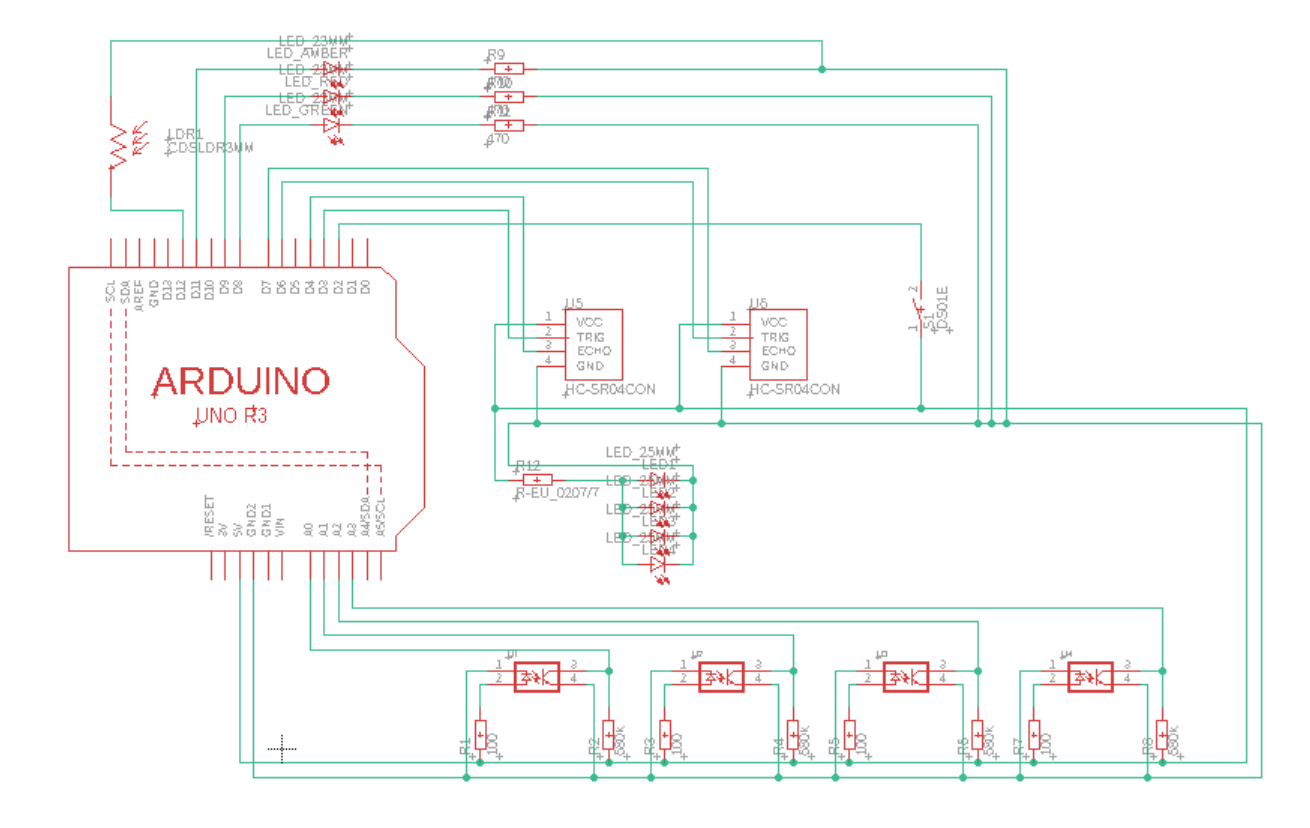
\includegraphics[width=0.8\textwidth]{assets/Schematic.png}
    \caption{Component Schematic}
    \label{fig:schematic}
\end{figure} 

\quad These were all done soldering in week 3 and ready for test on stripboard. We originally used stripboard to build our circuit as it is faster to prototype and change any designs according to tested results. Functions are all tested fine before installed to the robot. As the four line sensors occupied all analog inputs on the arduino, we implemented code in software to make pin 12 capable of  reading analog inputs and have the LDR connected to it.

\quad However before the first competition, the board get shorted by the nuts on the robot, casued one of the line sensors not working. This has been the major reason for scoring 20 in the first competition, as the robot lost its ability to navigated back. After that test, we decided to change to the Arduino protoboard as most of the design are settled and it is apparently more stable. This is the protoboard design we’ve raised:

\begin{figure}[!h]
    \centering
    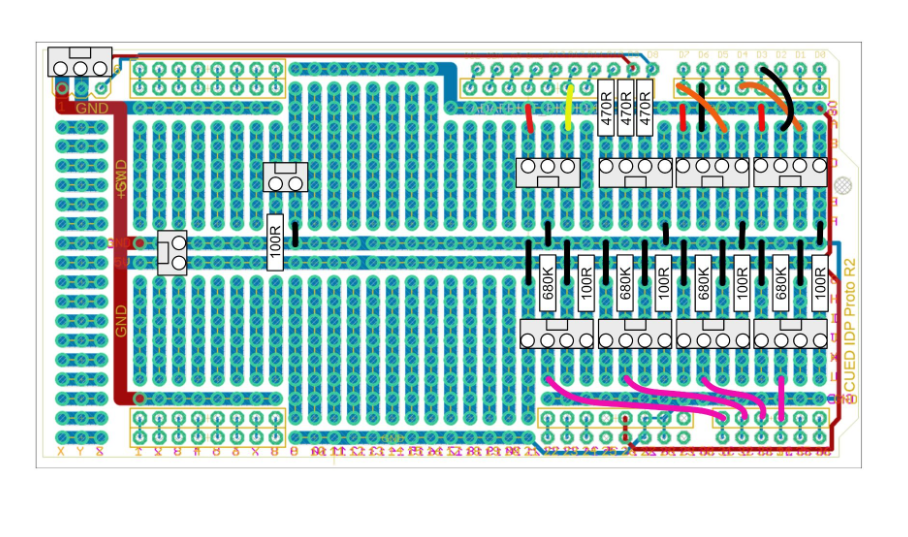
\includegraphics[width=0.8\textwidth]{assets/Proto.png}
    \caption{Board layout}
    \label{fig:board_layout}
\end{figure} 

\begin{figure}[!h]
    \centering
    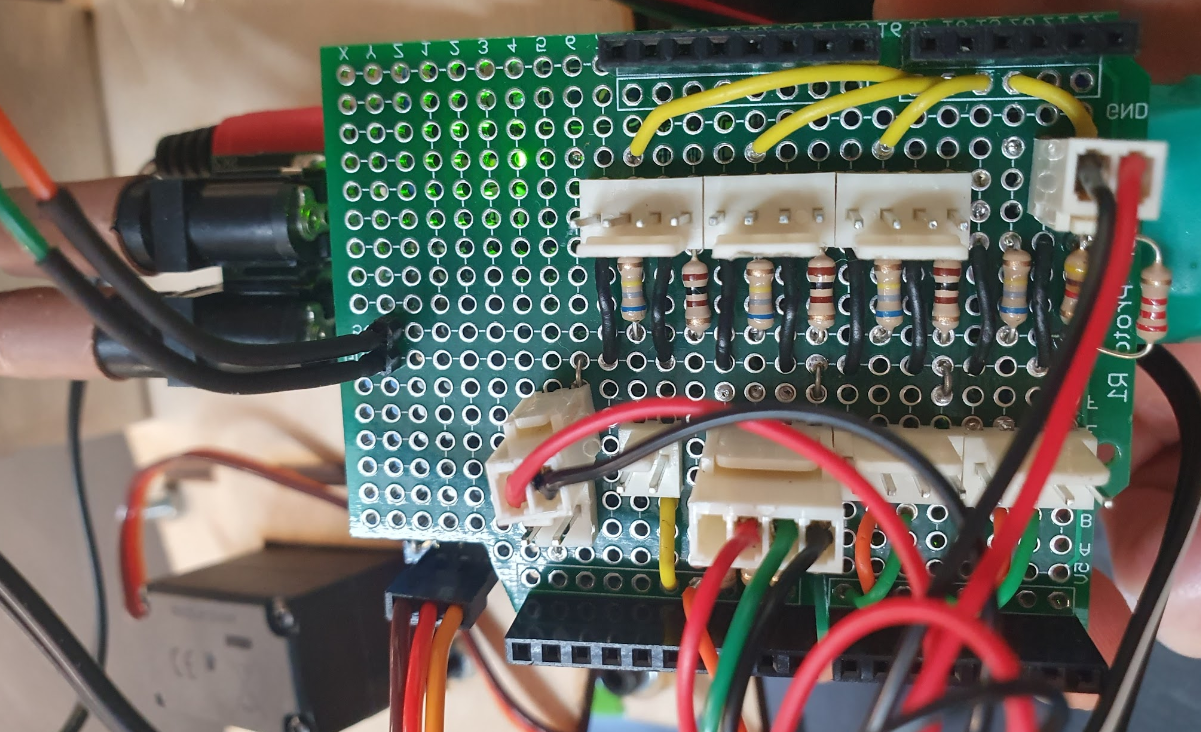
\includegraphics[width=0.8\textwidth]{assets/Board.png}
    \caption{Soldered protoboard}
    \label{fig:final_board}
\end{figure} 

\subsection{OpenCV}
\quad Before week 4 we get OpenCV working, and therefore we decided to switch to OpenCV navigation approach. As OpenCV is uncapable of block detection, the detection mechanism has been kept. Line sensors and ultrasonic sensors are no longer required, and the updated component list is as follow:

\quad The only change to the PCB is LDR now connected to A4 to ensure stable performance, as line sensors no longer required. Besides that, while components are mostly removed, the sockets are kept on the protoboard, so no other design has changed.

\section{Software}

\quad The software team consists of Yian.W (yw543) and Yuge.Z (yz754). We plan to employ finite state machine to drive the overall flow, and identified four main procedures that we would work on for the project, namely line following, distance tracking(below tunnel), block detection and pick-up/lay-off as seen below. 
\begin{figure}[!h]
    \centering
    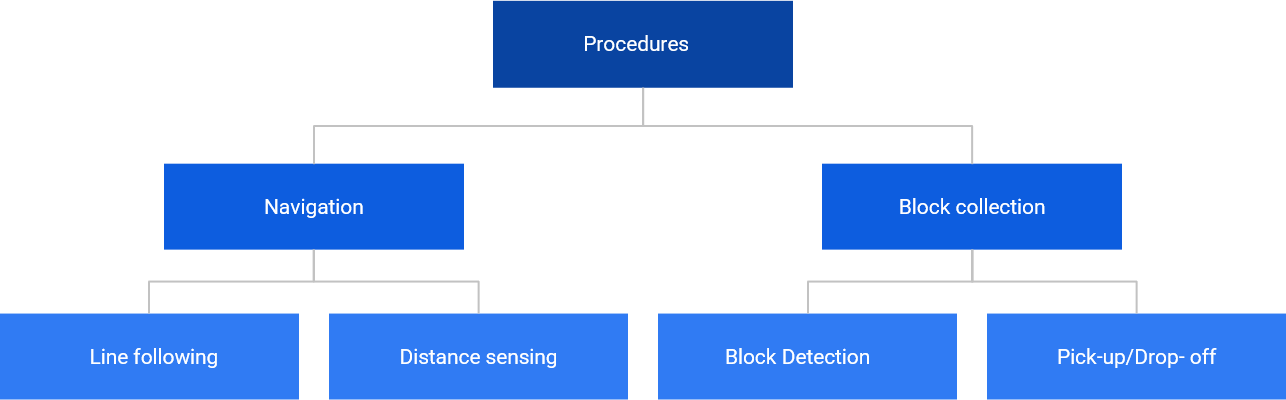
\includegraphics[width=0.8\textwidth]{assets/software_overview.png}
    \caption{Software Overview}
    \label{fig:software_overview}
\end{figure} 

\subsection{Exploration and navigation alogrithms}
\quad quad Our group decided on using the line-following method to navigate the robot. By placing 3 OPB sensors, we could obtain different analog reading values corresponding to the color of the surfaces under various scenarios. Specifically with regards to interface to electronics, high voltage readings correspond to black surfaces, and lower voltage readings correspond to that of white line, allowing deviation from the line to be detected. We could change outputs as that of the speed of each motor, such that it would make necessary adjustments/turns under different scenarios. 

\quad In addition, we plan to use inputs from an ultrasonic sensor to determine the distance from one side of the wall, and maintain navigation process when there is no line to follow beneath the tunnel. 

\subsection{Block collection algorithms}
\quad Block collection could be broken down into two main stages: detection of the density of the block and pick-up/lay-off procedure. The block detection stage will be initiated when a distance sensor placed at the front read a value beneath a particular threshold, e.g. 5cm. To determine the density of the block, the ultrasonic sensor is used to produce analog readings that correspond to high/low density block. The outputs would be the ledstate of pins corresponding to the red/green LED respectively. Upon flashing signals, the pick-up procedure would be initiated and a PWM signal would be sent as an output to the Servo to clamp the block. The lay-off procedure is similar. 

% Yuge and Steve please fill in your work here %
\subsection{OpenCV}
\subsubsection{Overall Plan}
This branch of the project is currently in the nightly stage, i.e. we are only exploring the feasibility of using computer vision, powered by the OpenCV library, to carry out path planning around the arena and therefore offloading the navigation of the robot entirely to a PC.

Should this be successful, the overall operation would involve streaming the live video feed from the overhead webcams into a Python script, which would carry out the following processing steps:
\begin{enumerate}
    \item World Mapping 
    \begin{description}[leftmargin=-0.2in]
        \item The script would detect all the features within the field of view such as the white path lines, the red and green squares, and the lime colored obstacle. A map of the arena would be constructed from the location information of these features, and cached into memory.
    \end{description}
    \item Navigate to Payload
    \begin{description}[leftmargin=-0.2in]
        \item[] In this state, the script waits for the presence of the target payload (the foam blocks). Once a foam block is detected, a pathfinding algorithm would be run to establish a path from the current robot position to the position of the foam blocks. Commands will then be sent to the robot to move according to the aforementioned path.
    \end{description}
    \item Navigate to Goal Area
    \begin{description}[leftmargin=-0.2in]
        \item[] In a similar manner, once the foam block has been picked up and it's category determined, the path planning algorithm infers a path from the current robot position to the goal area. Commands will then be sent to the robot to carry out the required movements.
    \end{description}
\end{enumerate}

We plan to use UDP packets to stream commands to the Arduino on the robot, which would be configured to be an access point so that we have a dedicated data pipe that will not be affected by inconsistencies of the network infrastructure in the department. However, should the handling of the UDP packets become too much of a challenge, we could fall back to sending HTTP requests to command the Arduino - an approach that has been well documented by others within the maker community.

\subsubsection{Potential Issues and Ways to Mitigate Them}
\begin{enumerate}
    \item Latency
    \begin{description}[leftmargin=-0.2in]
        \item[] We noticed that OpenCV buffers frames as they come in over the MJPEG stream, and therefore, with our current naive implementation, the speed at which the processing loop runs determines how much the current frame being processed lags behind real time.
        \item[] This should be an easy fix, a thread could be spawned to clear out the frame buffer such that the current frame being read by the processing loop is never stale.
    \end{description}
    \item Network Dropout
    \begin{description}[leftmargin=-0.2in]
        \item[] We were informed multiple times by various parties that network stability was a huge issue for teams in the past.
        \item[] In the event that issues with 802.11b/g/n network congestion become significant, the ESP32 on board the Arduino also has native support for Bluetooth Low Energy (BLE), which implements frequency hopping specifically to combat congestion, so we would switch over to using BLE for communication between the PC and the Arduino.
    \end{description}
\end{enumerate}


\section{Appendix}
% Please put all of your image documents in the asset folder and place all of your figures here. TQ

\begin{figure}[!h]
    \centering
    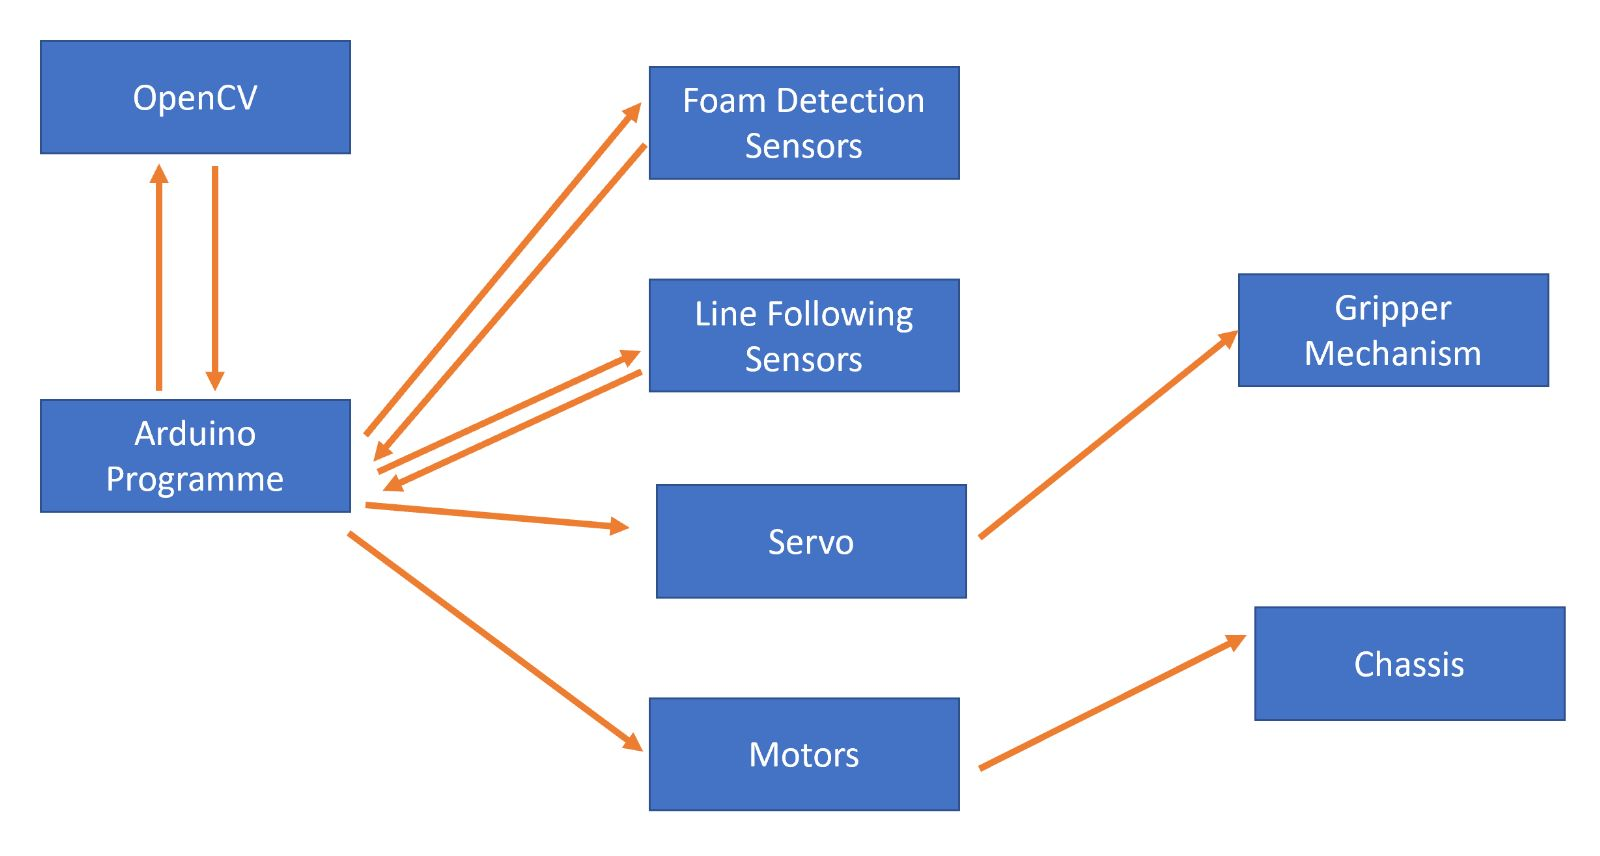
\includegraphics[width=0.8\textwidth]{assets/Overall_sys.jpg}
    \caption{Overall System Level Diagram}
    \label{fig:overall_sys}
\end{figure}

\begin{figure}[!h]
    \centering
    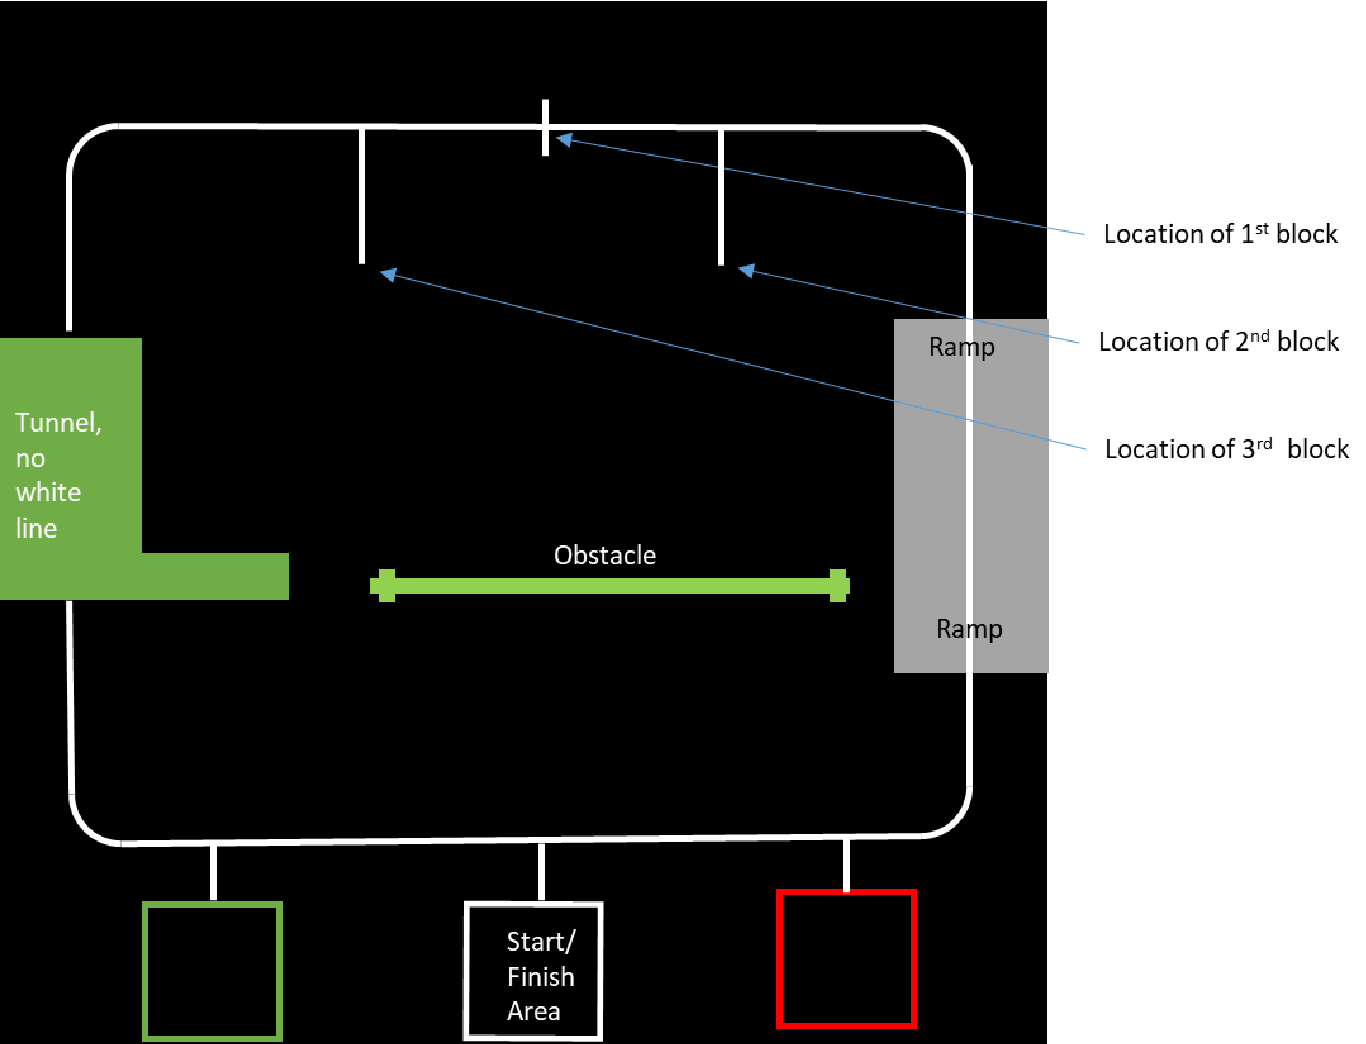
\includegraphics[width=0.8\textwidth]{assets/arena.png}
    \caption{Arena layout}
    \label{fig:arena}
\end{figure}

\begin{figure}[!h]
    \centering
    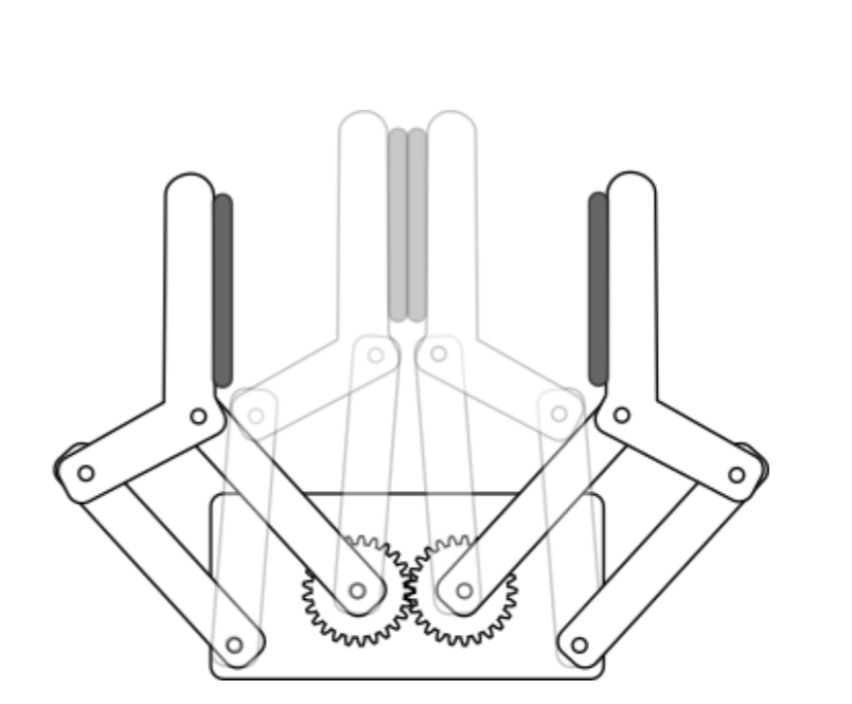
\includegraphics[width=0.8\textwidth]{assets/Gripper_Mechanism.jpg}
    \caption{Scissor-like Gripper Mechanism}
    \label{fig:grip_mech}
\end{figure}

\begin{figure}[!h]
    \centering
    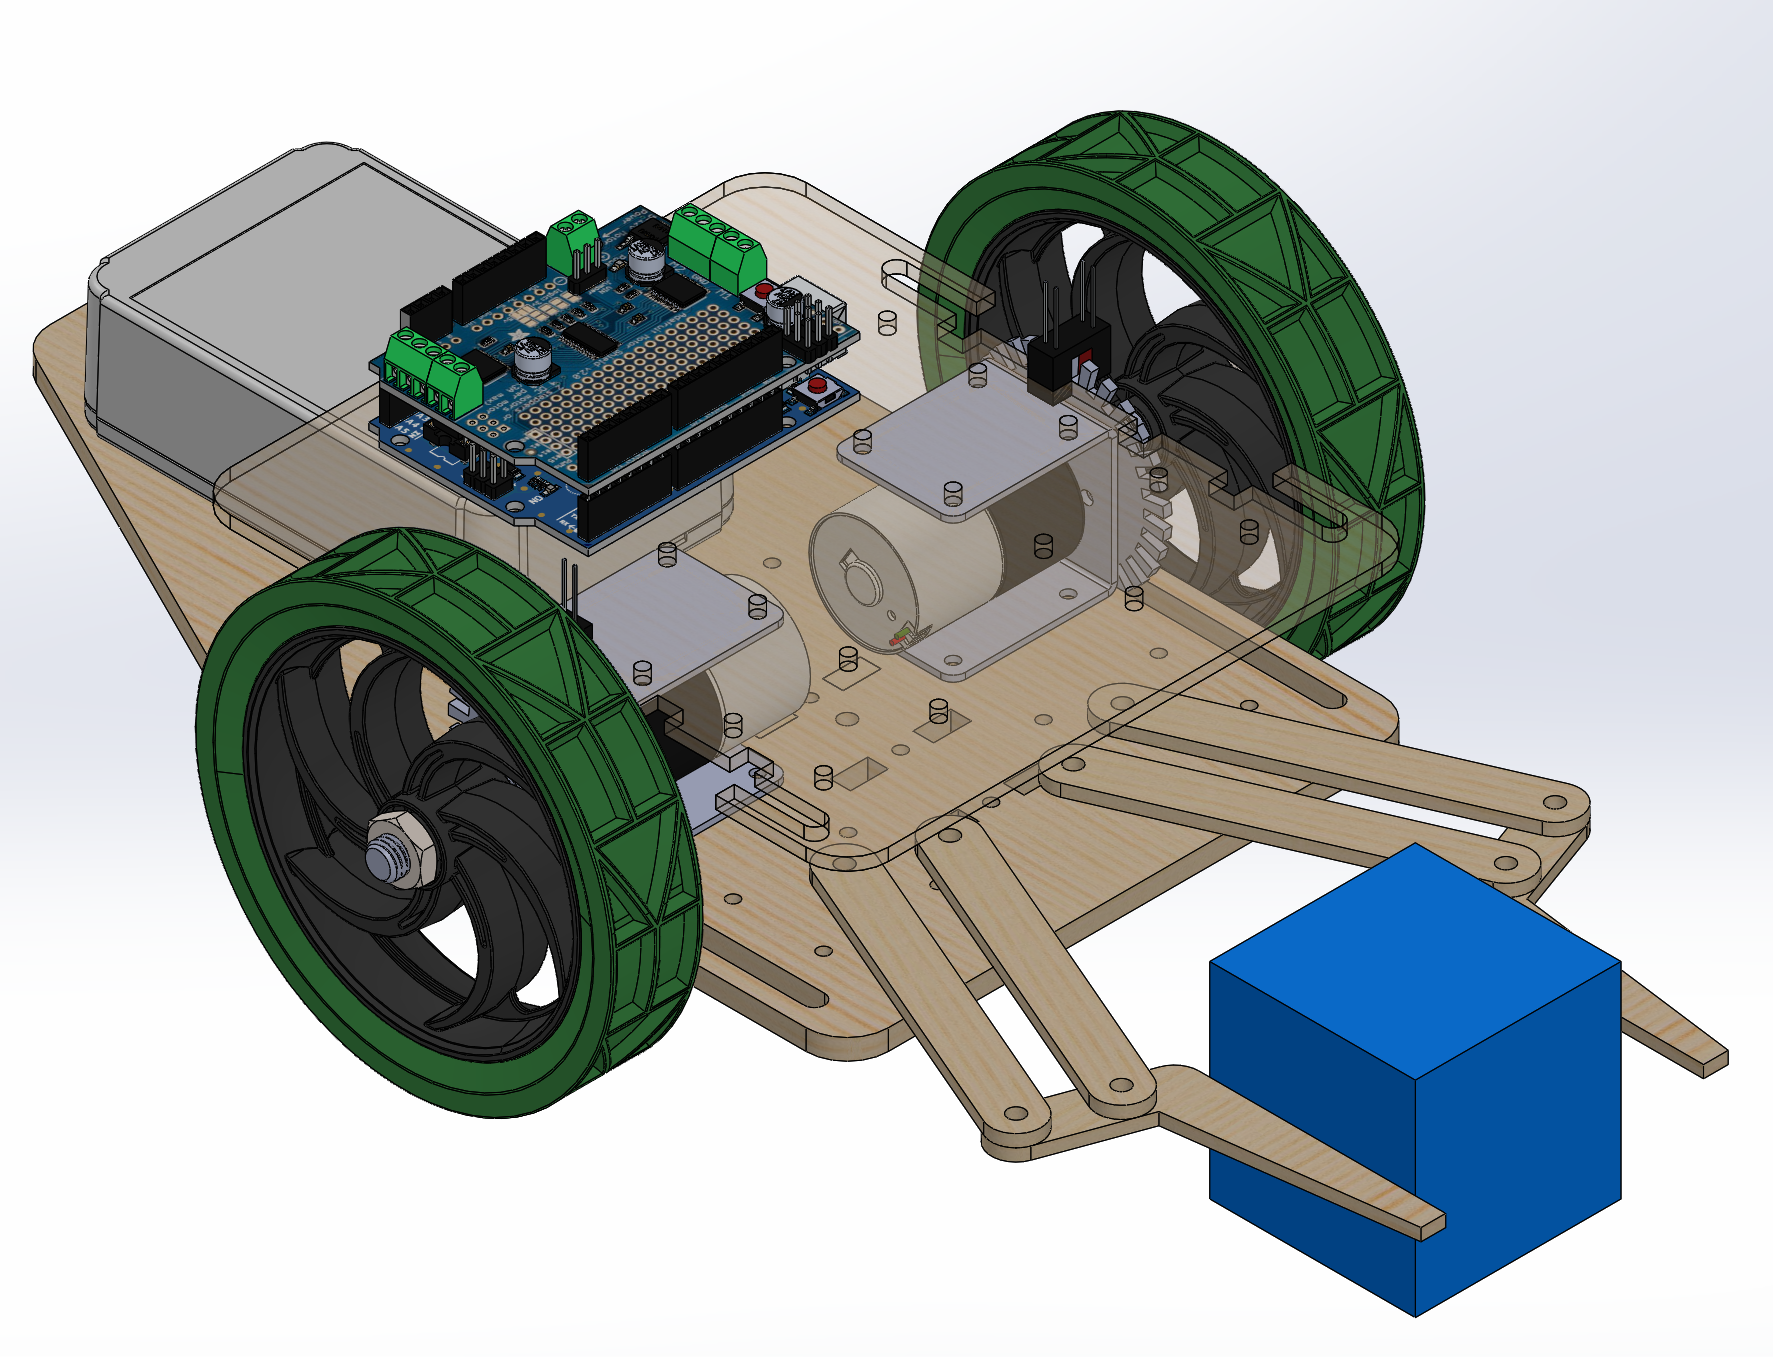
\includegraphics[width=0.8\textwidth]{assets/isometric.png}
    \caption{Current Isometric Solidworks Model}
    \label{fig:isometric}
\end{figure}

\begin{figure}[!h]
    \centering
    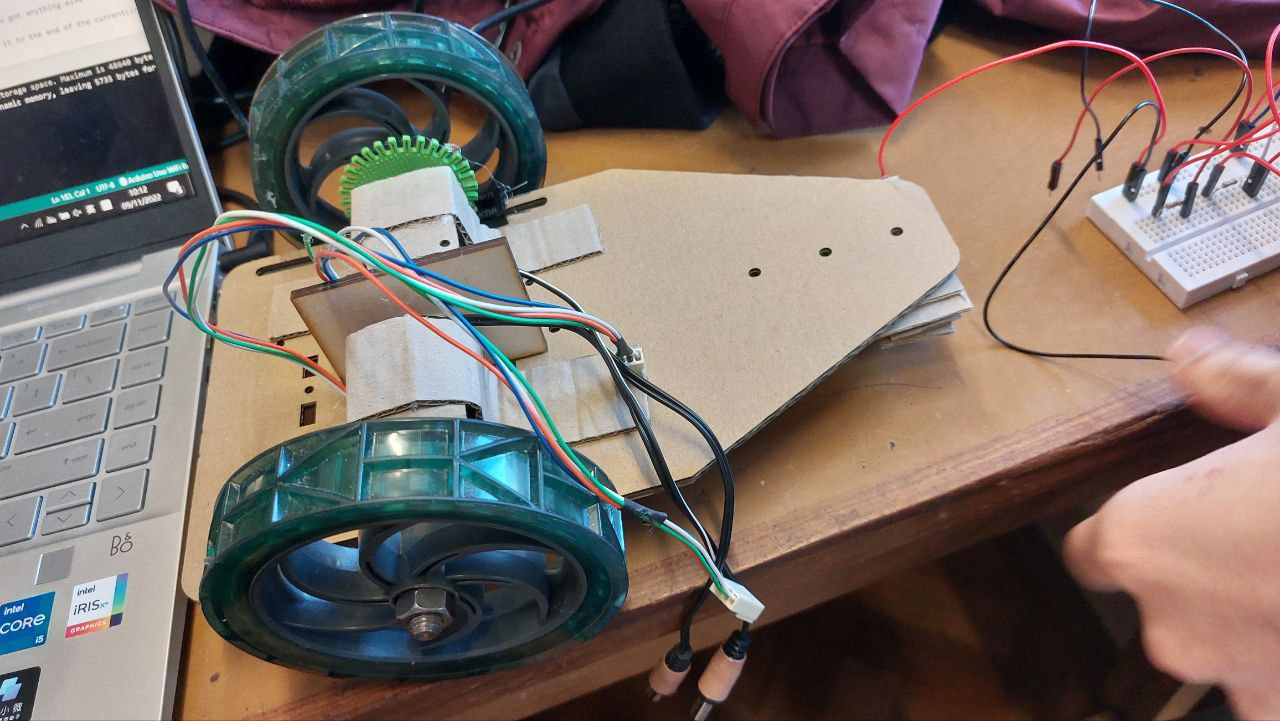
\includegraphics[width=0.8\textwidth]{assets/Cardboard_model.jpg}
    \caption{Cardboard Model}
    \label{fig:cardboard_model}
\end{figure}

\begin{figure}[!h]
    \centering
    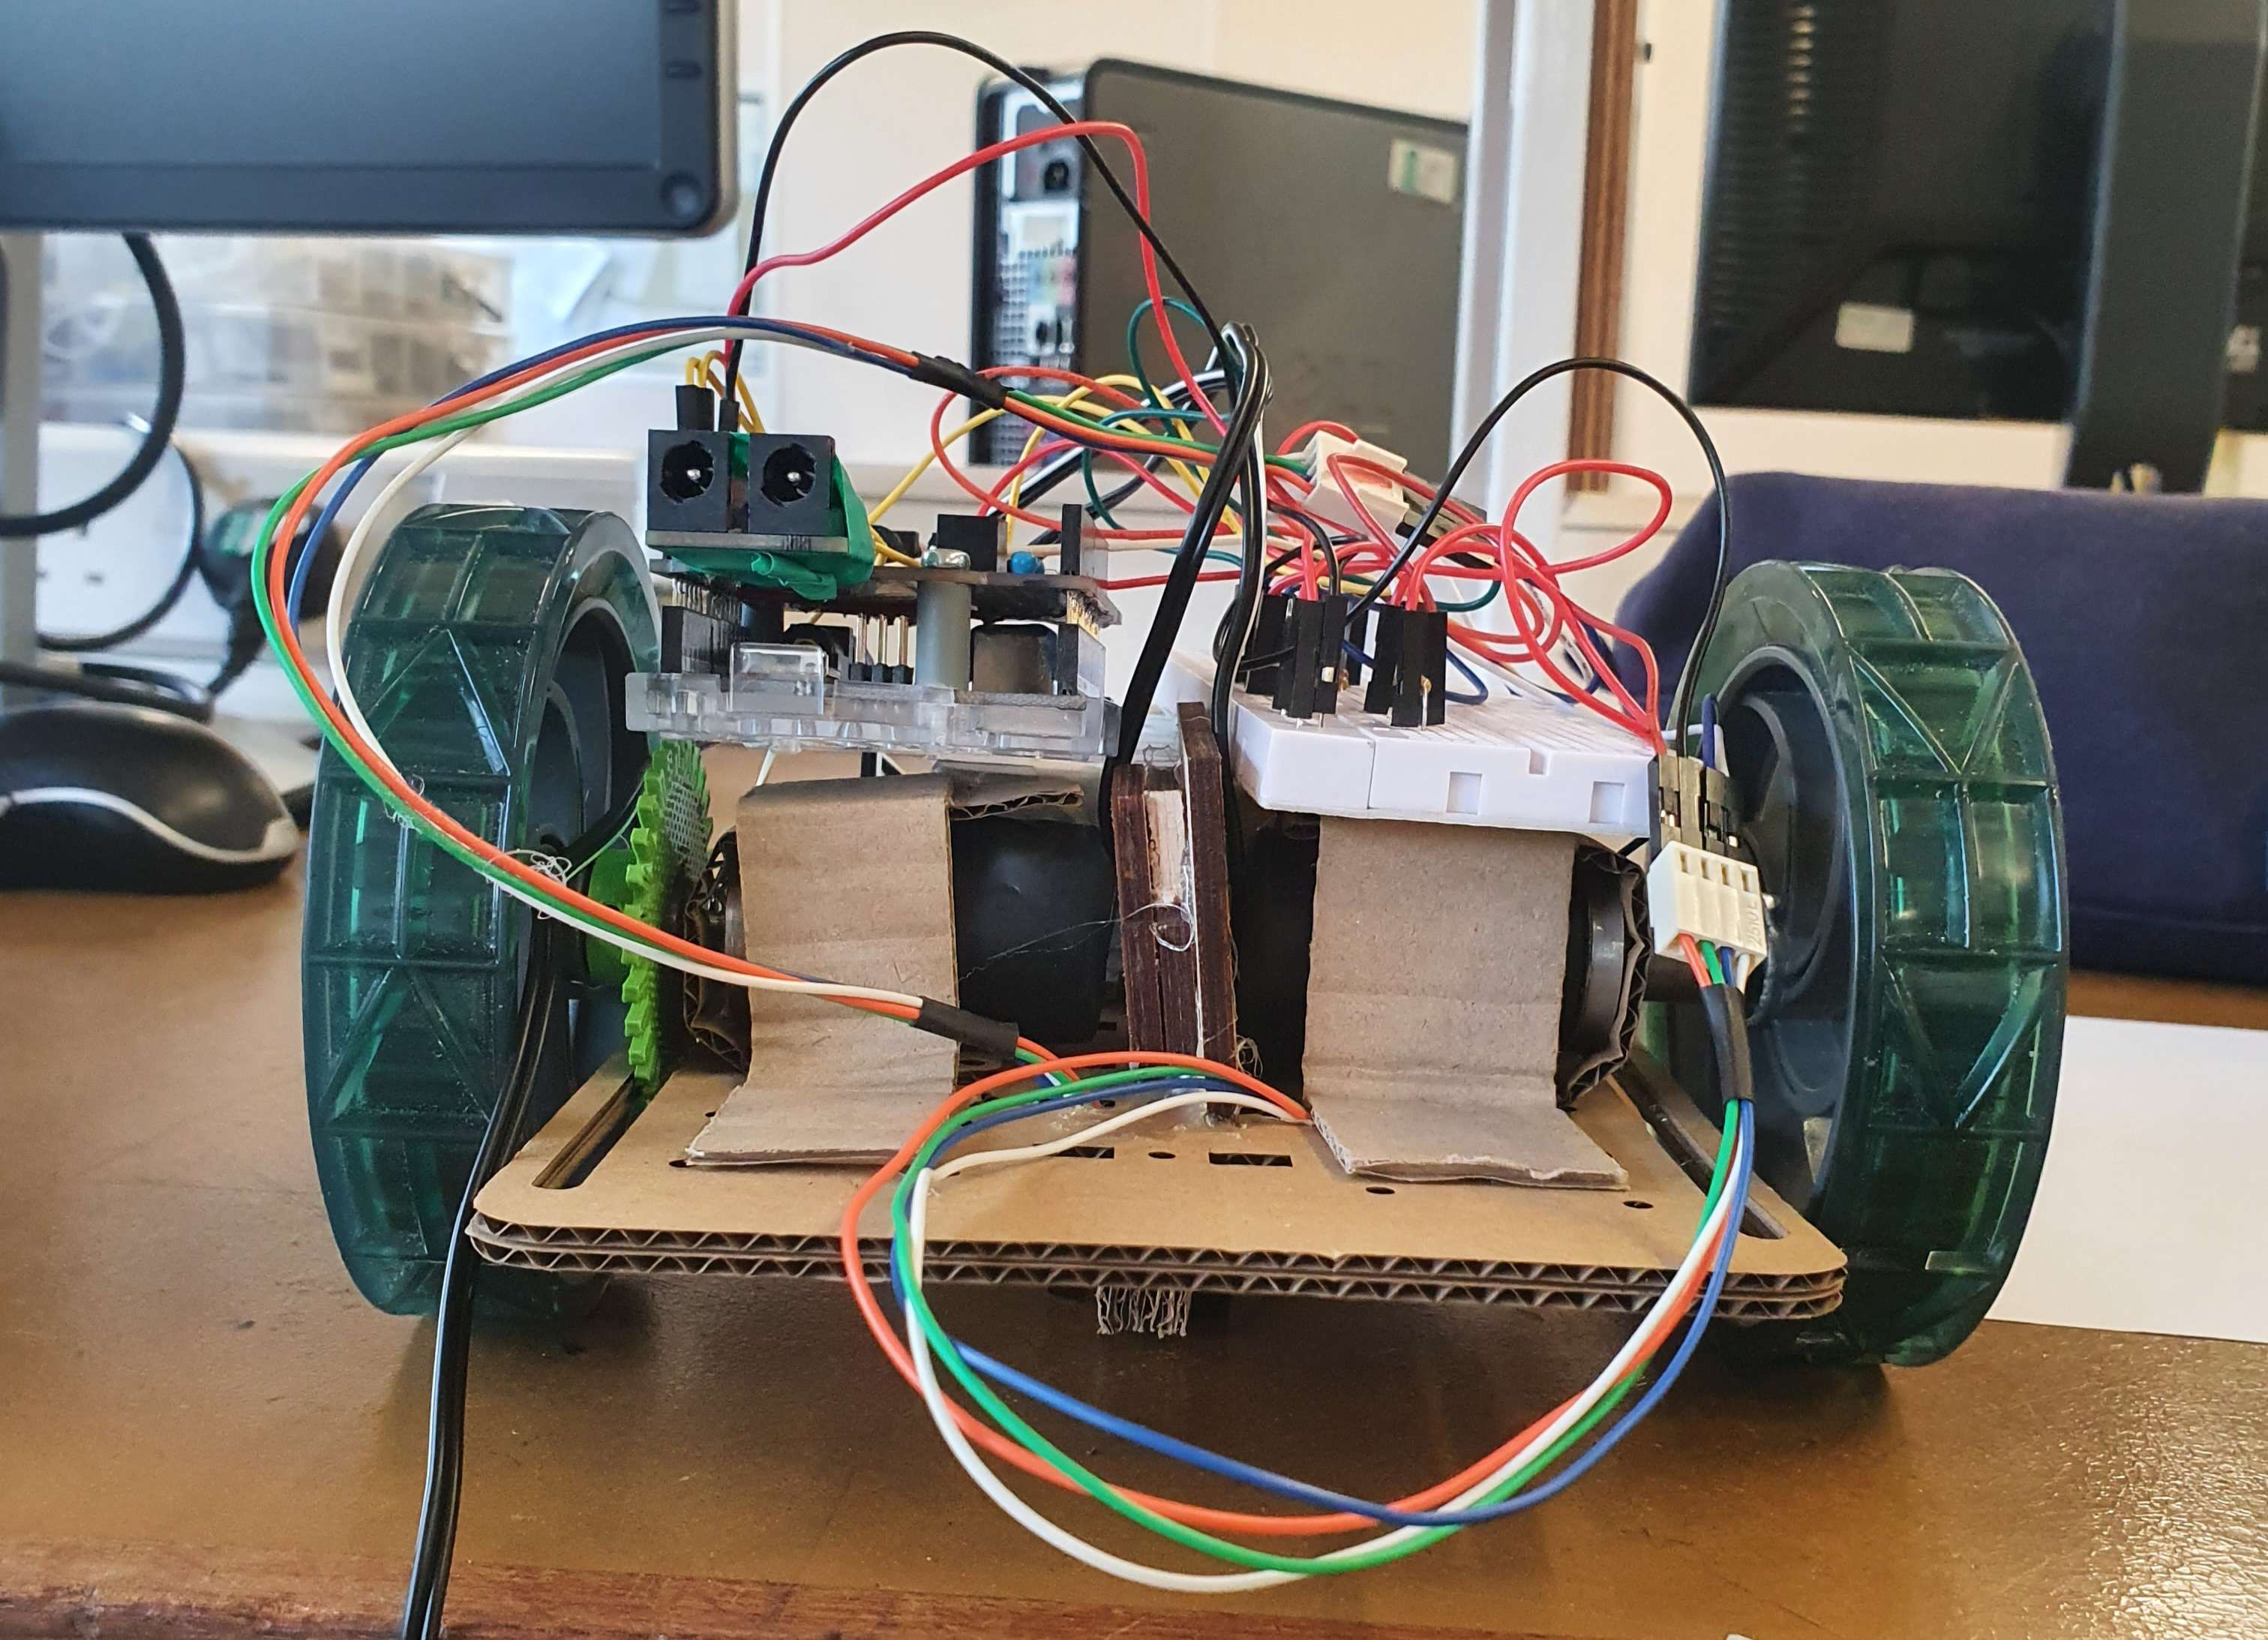
\includegraphics[width=0.8\textwidth]{assets/assembled_prototype.jpg}
    \caption{Assembled Prototype}
    \label{fig:assembled_prototype}
\end{figure}



\end{document}
